\lab{Algorithms}{Ising Model}{Ising Model}
\objective{Understand how to use the Metropolis algorithm to calculate Ising model estimations.}

The Ising model is a mathematical model in statistical mechanics. It describes how atoms interact in ferromagnetic material. More specifically, we assume that there is some lattice $\Lambda$ of sites. We say $i \sim j$ if $i$ and $j$ are adjacent sites. With each site $i$ in our lattice is an associated \emph{spin} $\sigma_{i} \in \{\pm 1\}$. A \emph{state} in our Ising model is a particular spin configuration $\sigma = (\sigma_{j})_{j \in \Lambda}$. If $L = |\Lambda|$, then there are $2^{L}$ possible states in our model. If $L$ is large, the state space becomes huge, which is why Bayesian sampling methods (in particular the Metropolis algorithm) are so useful in calculating model estimations.

With any spin configuration $\sigma$, there is an associated energy $H(\sigma) = -J \sum_{i \sim j} \sigma_{i} \sigma_{j}$ where $J > 0$ for ferromagnetic materials, and $J < 0$ for antiferromagnetic materials. Throughout this lab, we will assume $J = 1$, leaving the energy equation to be $H(\sigma) = -\sum_{i \sim j} \sigma_{i}\sigma_{j}$ where the interaction from each pair is added only once.

We will consider a lattice that is a $100 \times 100$ square grid. The adjacent sites for a given site are those directly above, below, to the left, and right of the site, so to speak. For sites on the edge of the grid, we assume it wraps around. In other words, a site at the furthest left of the grid is adjacent to the corresponding site on the furthest right. In this manner, the grid is actually a torus (this isn't really important, just kind of interesting). Thus, a single spin configuration can be represented as a $100 \times 100$ array, with entries from $\{\pm 1\}$.

\begin{problem}
Write a function that initializes a spin configuration for an $n \times n$ lattice. It should return an $n \times n$ array, each entry of which is either $1$ or $-1$, chosen randomly. Test this for the grid described above, and plot the spin configuration using \li{matplotlib.pyplot.imshow}. It should look fairly random, as below.
\end{problem}

\begin{figure}
\centering
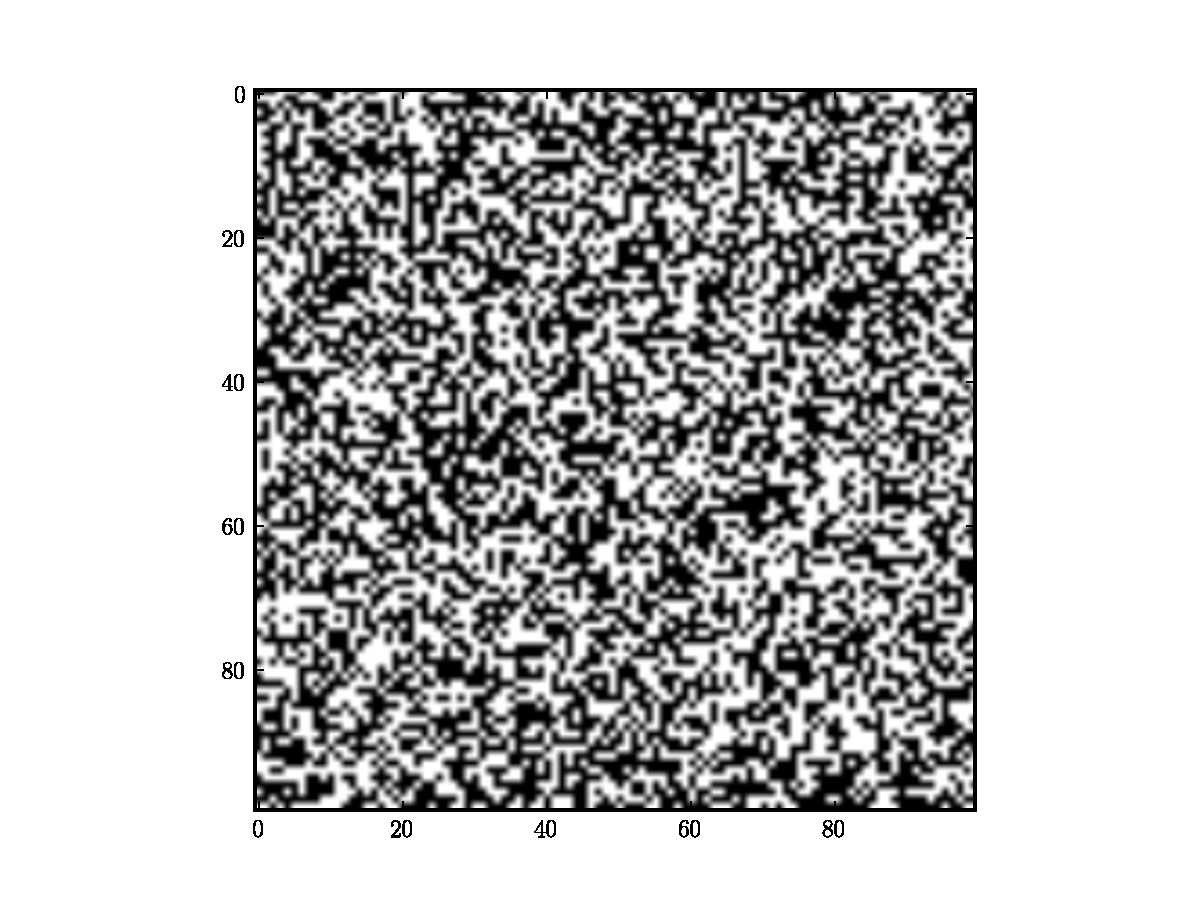
\includegraphics[width=\textwidth]{init.pdf}
\caption{Spin configuration from random initialization.}
\end{figure}

\begin{problem}
Write a function that computes the energy of a spin configuration with an $n \times n$ lattice described above. Make sure that you do not double count site pair interactions!
\end{problem}

Different spin configurations occur with different probabilities, depending on the energy of the spin configuration and $\beta > 0$, an inverse function of temperature. More specifically, for a given $\beta$, we have
\begin{equation*}
\mathbb{P}_{\beta}(\sigma) = \frac{e^{-\beta H(\sigma)}}{Z_{\beta}}
\end{equation*}
where $Z_{\beta} = \sum_{\sigma} e^{-\beta H(\sigma)}$. Because for our particular lattice there are $2^{100 \cdot 100} = 2^{10000}$ possible spin configurations, computing this sum is unfeasible. However, the numerator is quite simple, provided we can efficiently compute the energy $H(\sigma)$ of a spin configuration. Thus the ratio of the probability densities of two spin configurations is simple: 
\begin{align*}
\frac{\mathbb{P}_{\beta}(\sigma^{*})}{\mathbb{P}_{\beta}(\sigma)} & = \frac{e^{-\beta H(\sigma^{*})}}{e^{-\beta H(\sigma)}} \\
& = e^{\beta (H(\sigma) - H(\sigma^{*}))}
\end{align*}

The simplicity of this ratio should lead us to think that a Metropolis algorithm might be appropriate by which to sample from the spin configuration probability distribution, in which case our acceptance probability would be
\begin{equation*}
A(\sigma^{*} | \sigma) = \begin{cases} 1 & \mbox{if } H(\sigma^{*}) < H(\sigma) \\ e^{\beta (H(\sigma) - H(\sigma^{*}))} & \mbox{ otherwise.} \end{cases}
\end{equation*}

By choosing our transition matrix $Q$ cleverly, we can also make it easy to compute the energy for any proposed spin configuration. We restrict our possible proposals to only those spin configurations in which we have flipped the spin at exactly one lattice site, i.e. we choose a lattice site $i$ and flip its spin. Thus, there are only $L$ possible proposal spin configurations $\sigma^{*}$ given $\sigma$, each being proposed with probability $\frac{1}{L}$, and such that $\sigma_{j}^{*} = \sigma_{j}$ for all $j \neq i$, and $\sigma_{i}^{*} = - \sigma_{i}$. Note that we would never actually write out this matrix (it would be $2^{10000} \times 2^{10000}$!!!). Computing the proposed sites energy is simple: if the spin flip site is $i$, then we have $H(\sigma^{*}) = H(\sigma) + 2\sum_{j: j \sim i} \sigma_{i}\sigma_{j}$.

\begin{problem}
Write a function that proposes a new spin configuration given the current spin configuration on an $n \times n$ lattice described above. This function simply needs to return a pair of indices $i,j$, chosen with probability $\frac{1}{n^{2}}$.
\end{problem}

\begin{problem}
Write a function that computes the energy of a proposed spin configuration, given the current spin configuration, its energy, and the proposed spin flip site indices.
\end{problem}

\begin{problem}
Write a function that accepts or rejects a proposed spin configuration, given the current configuration. It should accept the current energy, proposed energy, and $\beta$, and return a boolean.
\end{problem}

As in the last lab, we would like to look at the probabilities of each sample at each time. However, this would require us to compute the denominator $Z_{\beta}$, which as we explained previously is generally the reason we have to use a Metropolis algorithm to begin with. However, $Z_{\beta}$ is independent of any particular spin configuration, so we can just keep track of the numerator in the probability density function, which is $e^{-\beta H(\sigma)}$. In fact, we can take the log of this, and examine only $-\beta H(\sigma)$. We should see this increase as the algorithm proceeds, and converge once we are sampling from the correct distribution.

\begin{problem}
Write a function that initializes a spin configuration for an $n \times n$ lattice as done previously, and then performs the Metropolis algorithm, choosing new spin configurations and accepting or rejecting them. It should burn in first, and then iterate $n\_samples$ times, keeping every $100^{\text{th}}$ sample (this is to prevent memory failure) and all of the above values $-\beta H(\sigma)$ (keep the values even for the burn in period). It should also accept $\beta$ as an argument, allowing us to effectively adjust the temperature for the model. 
\end{problem}

\begin{problem}
Test your Metropolis sampler on a $100 \times 100$ grid, with $200000$ iterations, with $n\_samples$ large enough to get $50$ samples, testing with $\beta = 1$ and then with $\beta = 0.2$. Plot the proportional log probabilities, and also plot a late sample from each test using \li{matplotlib.pyplot.imshow}. How does the ferromagnetic material behave differently with differing temperatures? Recall that $\beta$ is an inverse function of temperature. You should see more structure with lower temperature, as below.
\end{problem}

\begin{figure}
	\begin{subfigure}[b]{.49\textwidth}
		\centering
		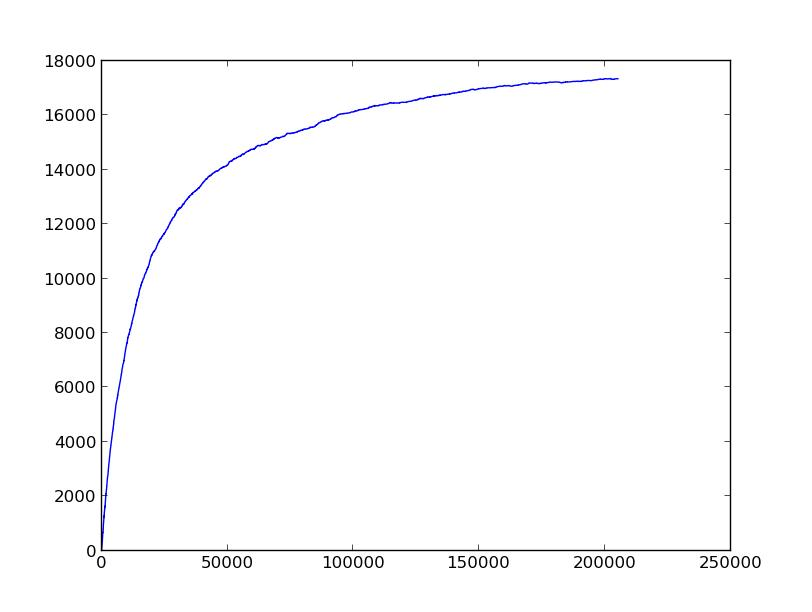
\includegraphics[width=\textwidth]{beta1_logprobs.jpeg}
		\caption{Proportional log probs when $\beta = 1$.}
		\label{figur:1}
	\end{subfigure}
	\begin{subfigure}[b]{.49\textwidth}
		\centering
		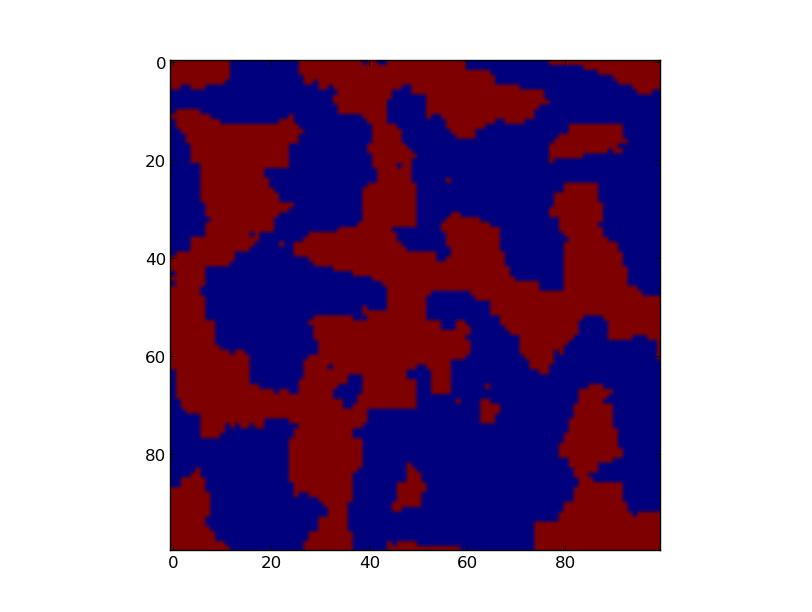
\includegraphics[width=\textwidth]{beta1_sample.jpeg}
		\caption{Spin configuration sample when $\beta = 1$.}
		\label{figur:2}
	\end{subfigure}
	\begin{subfigure}[b]{.49\textwidth}
		\centering
		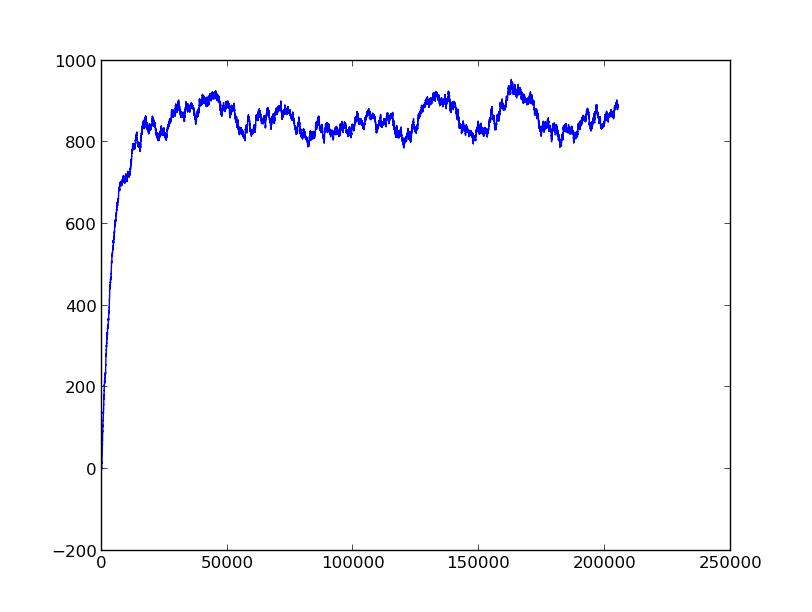
\includegraphics[width=\textwidth]{beta02_logprobs.jpeg}
		\caption{Proportional log probs when $\beta = 0.2$.}
		\label{figur:3}
	\end{subfigure}
	\begin{subfigure}[b]{.49\textwidth}
		\centering
		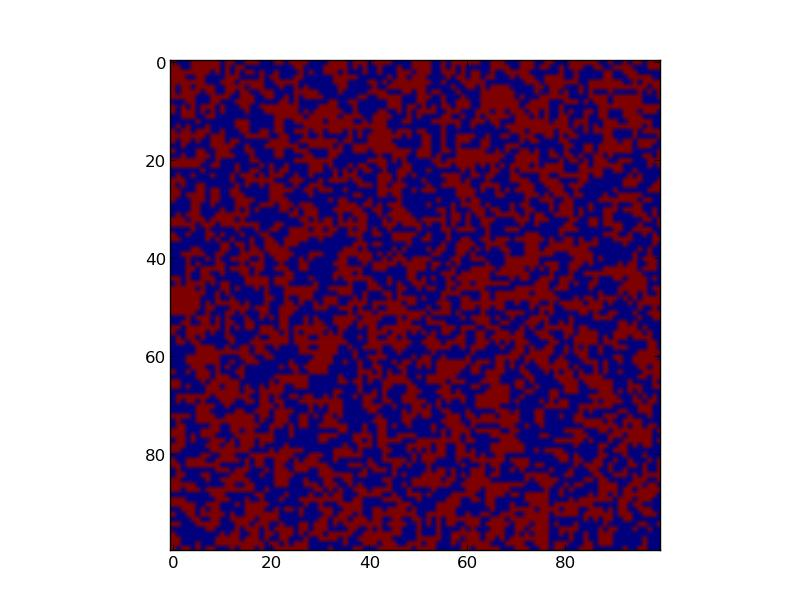
\includegraphics[width=\textwidth]{beta02_sample.jpeg}
		\caption{Spin configuration sample when $\beta = 0.2$.}
		\label{figur:4}
	\end{subfigure}
\end{figure}